\section{Preverjanje predpostavk linearnega regresijskega modela}\label{sec5}

Predpostavke linearnega regresijskega modela bomo preverili s pomočjo štirih \emph{diagnostičnih grafov}.
Če nekatere predpostavke nisi izpolnjene so lahko rezultati netočni.

\begin{figure}[!h]
    \centering
    \begin{subfigure}[ht]{0.49\textwidth}
        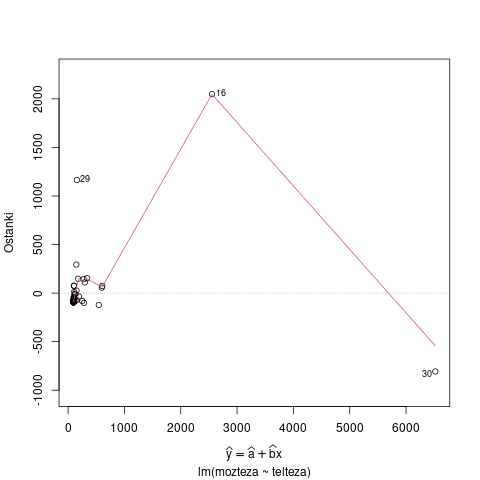
\includegraphics[width=\textwidth]{res/linearnost-modela.png}
        \caption{Linearnost modela}
        \label{img:linearnost-modela}
    \end{subfigure}
    \hfill
    \begin{subfigure}[ht]{0.49\textwidth}
        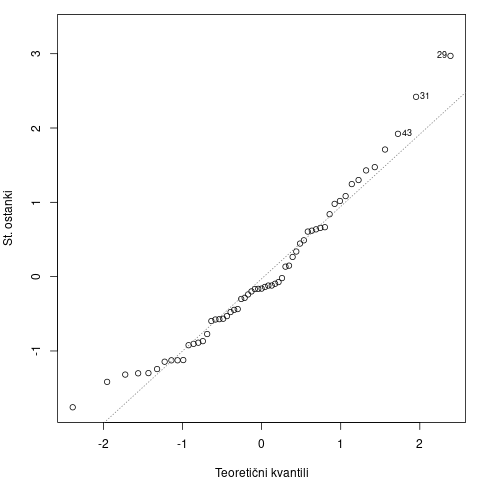
\includegraphics[width=\textwidth]{res/normalnost-porazdelitve.png}
        \caption{Normalnost porazdelitve}
        \label{img:normalnost-porazdelitve}
    \end{subfigure}

    \begin{subfigure}[ht]{0.49\textwidth}
        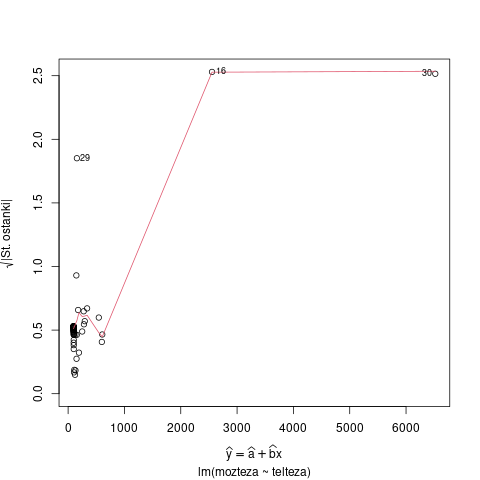
\includegraphics[width=\textwidth]{res/homogenost-variance.png}
        \caption{Homogenost variance}
        \label{img:homogenost-variance}
    \end{subfigure}
    \hfill
    \begin{subfigure}[ht]{0.49\textwidth}
        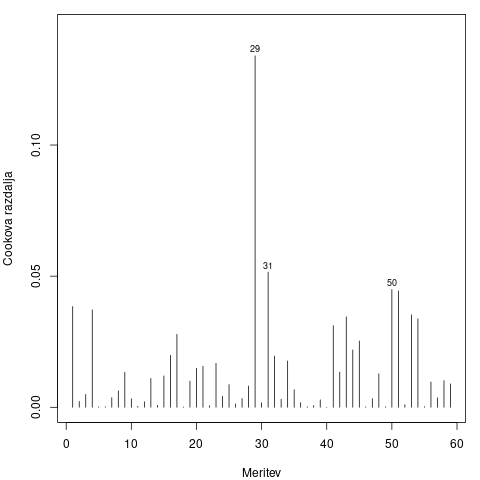
\includegraphics[width=\textwidth]{res/vpliv-tock-na-model.png}
        \caption{Vpliv točk na model}
        \label{img:vpliv-tock-na-model}
    \end{subfigure}
    \caption{Diagnostični grafi}
    \label{img:diagnosticni-grafi}
\end{figure}

\newpage

\noindent
Diagnostične grafe smo generirali s spodnjo kodo:

\begin{verbatim}
    xlgteza = data.frame(lgtteza = log(c(100, 500, 2000)))
    predict(model, xlgteza, interval = "predict")
    
    png("linearnost-modela.png")
    par(mar=c(4,4,1,1))
    plot(model, which = 1, caption = "", ann = F)
    title(
        xlab = expression(widehat(y) == widehat(a) + widehat(b) * x),
        ylab = "Ostanki"
    )
    dev.off()
    
    png("normalnost-porazdelitve.png")
    par(mar=c(4,4,1,1))
    plot(model, which = 2, caption = "", ann = F)
    title(xlab = "Teoretični kvantili", ylab = "St. ostanki")
    dev.off()
    
    png("homogenost-variance.png")
    par(mar=c(4,4,1,1))
    plot(model, which = 3, caption = "", ann = F)
    title(
        xlab = expression(widehat(y) == widehat(a) + widehat(b) * x),
        ylab = expression(sqrt(paste("|St. ostanki|")))
    )
    dev.off()
    
    png("vpliv-tock-na-model.png")
    par(mar=c(4,4,1,1))
    plot(model, which = 4, caption = "", ann = F)
    title(xlab = "Meritev", ylab = "Cookova razdalja")
    dev.off()
\end{verbatim}

\noindent
Za izris grafov v funkciji \emph{plot()} izberemo linearni regresijski model iz katerega želimo izrisati grafe
(v našem primeru \emph{model}), da ne želimo prikazati naslova (\verb|caption = ""|) in ann (\verb|ann = F|),
v funkciji \emph{title()} pa izberemo podatke za besedilo x in y osi.

\subsection{Graf za preverjanje linearnosti modela}

Pravilnost linearnega regresijskega modela smo preverili z grafom ostankov v odvisnosti od \emph{x} vrednosti ali od
predvidenih vrednosti $\widehat{y} = \widehat{a}x + \widehat{b}$ in preverimo, če obstaja vzorec.
Če so točke vsaj približno enakomerno raztresene nad in pod premico \verb|Ostanki = 0| in ne moremo zaznati neke oblike
je linearni model pravilen.
Če opazimo kakšen vzorec, nam lahko oblika le-tega da informacijo o funkciji \emph{x}-a, ki manjka v modelu.

Ker za naše podatke na grafu ne opazimo vzorca lahko zaključimo, da je linearni model validen.
Točke na grafu ne zgledajo popolnoma naključno razporejene, ker lahko opazimo malo večjo koncentracijo točk za
predvidene vrednosti od 2 do 4, kar lahko pripišemo originalnim vrednostim naših podatkov
(glej Graf \ref{img:razs-diag}).

\subsection{Graf normalnosti porazdelitve naključnih napak}

Normalnost porazdelitve naključnih napak preverjamo preko grafa porazdelitve standardiziranih
ostankov. Ostanek se standardizira tako, da se deli z oceno njegovega standardnega odklona
(njegovo matematično upanje je 0).
Na \emph{x}-osi \emph{Q - Q} grafa normalne porazdelitve so podani teoretični kvantili, na \emph{y}-osi pa kvantili
standardiziranih ostankov.
Če dobljene točke na \emph{Q - Q} grafu tvorijo premico (z manjšimi odstopanji), zaključimo, da je porazdelitev
naključnih napak (vsaj približno) normalna.
Za podatke o telesni in možganski teži sesalcev lahko zaključimo, da so naključne napake normalno porazdeljene
(ni večjih odstopanj od premice, razen za 29., 31. in 43. podatkovno točko).

\subsection{Graf homogenosti variance}

Osnovna predpostavka linearnega regresijskega modela je, da imajo naključne napake konstantno homogenost variance.
Za registriranje nekonstantne variance uporabimo graf korena standardiziranih ostankov v odvisnosti od \emph{x}
ali od predvidenih vrednosti $\widehat{y} = \widehat{a}x + \widehat{b}$.
Če variabilnost korena standardiziranih ostankov narašča ali pada s povečanjem vrednosti $\widehat{y}$, je to znak,
da varianca naključnih napak ni konstantna.
Pri ocenjevanju lahko pomaga funkcija glajenja, pri kateri se v primeru konstantne variance pričakuje horizontalna
črta, okoli katere so točke enakomerno razporejene.
Za naše podatke, na osnovi grafa Homogenosti variance (glej graf \ref{img:homogenost-variance}), vidimo, da ni
naraščanja ali padanja variance.
Ničelno domnevo konstantne variance lahko preverimo s pomočjo testa konstantnosti variance (Breusch-Pagan test).

To storimo z ukazom \verb|ncvTest(model)|, pri čemer smo funkcijo \emph{ncvTest()} pridobili iz R paketa \emph{car}.
Dobimo rezultate:

\begin{verbatim}
    Non-constant Variance Score Test 
    Variance formula: ~ fitted.values 
    Chisquare = 0.5732155, Df = 1, p = 0.44898
\end{verbatim}

Na osnovi rezultata testa (testna statistika $\chi^{2} = 0.5732155$, df $= 1$, p-vrednost p = $0.44898 > 0.05$),
lahko sprejmemo ničelno domnevo, da je varianca naključnih napak konstantna.

\subsection{Graf vpliva posameznih točk na model}

Za merjenje vpliva \emph{i}-te točke na linearni regresijski model uporabimo \emph{Cookovo razdaljo}, definirano kot

\begin{equation}
    D_{i} = \frac{\sum_{j=1}^{n} (\widehat{Y}_{j(i)} - \widehat{Y_{j}})^{2}}{S^{2}},
\end{equation}

kjer je $\widehat{Y}_{j} = \widehat{a} + \widehat{b}X_{j}$ \emph{j}-ta predvidena vrednost in S ocena standardnega
odklona naključnih napak.
Z $\widehat{Y}_{j(i)}$ smo označili \emph{j}-to predvideno vrednost linearnega modela, ki je narejen brez \emph{i}-te
točke, na osnovi preostalih \emph{n - 1} točk.
Tako merimo razliko med modelom, ki vsebuje \emph{i}-to točko in modelom, ki je ne.
Če \emph{i}-ta točka ne vpliva močno na model, bo $D_{i}$ majhna vrednost.

Če je $D_{i} > \frac{4}{n - 2}$, kjer je \emph{n} velikost vzorca, potem \emph{i}-ta točka vpliva na linearni
regresijski model.
Če je tudi $D_{i} \geq c$, kjer je $c = F_{2,n - 2;0.5}$ mediana Fisherove porazdelitve z \emph{2} in \emph{n - 2}
prostorskima stopnjema, \emph{i}-ta točka močno vpliva na regresijski model.

Če imamo podatkovne točke z velikim vplivom na linearni regresijski model lahko naredimo naslednje,

\begin{itemize}
    \item Vprašamo se, če so podatki neobičajni ali drugačni od ostalih podatkov. V primeru da je odgovor pritrdilen,
    jih poskusimo odstraniti in konstruirati linearni model brez njih.
    \item Vprašamo se, če je linearni regresijski model validen za naše podatke. V primeru da opazimo, da bi podatkom
    bolj ustrezal kakšen drug model, ga probamo konstruirati, ali pa poskusimo s transformiranjem \emph{Y} ali \emph{X}.
\end{itemize}

Za naše podatke so osamelci, tri točke z najvišjo Cookovo razdaljo, 29., 31. in 50. podatkovna točka.
Da preverimo, če vplivajo na model, uporabimo ukaz

\noindent \verb|which(cooks.distance(model)>4/57)|, ki vrne rezultat \emph{29}.

Na modificiranem razsevnem diagramu (glej graf \ref{img:razsevni-diagram-pobarvan}) lahko opazimo, da je 29. podatkovna
točka, pobarvana modro, najbolj oddaljena od regresijske premice.
Da preverimo, ali je njen vpliv velik uporabimo ukaz

\noindent \verb|any(cooks.distance(model)[c(29)] >= qf(0.5, 2, 57))|,
ki nam vrne odgovor

\noindent \verb|[1] FALSE|, kar pomeni, da 29. podatkovna točka ne vpliva na linearni regresijski model,
zato je ni potrebno odstraniti.

\begin{figure}[h]
    \centering
    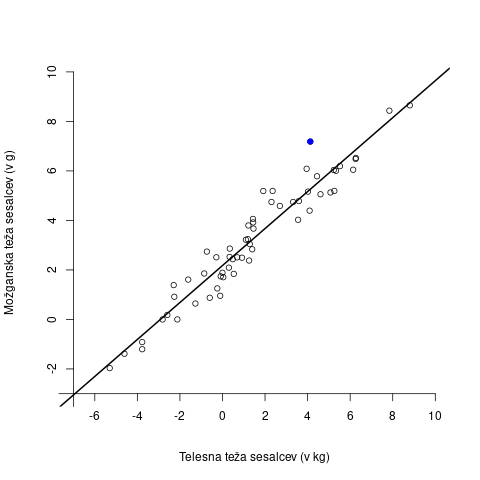
\includegraphics[scale=0.5]{res/razsevni-diagram-pobarvan.png}
    \caption{Razsevni diagram telesne in možganske teže sesalcev (s pobarvanimi osamelci)}
    \label{img:razsevni-diagram-pobarvan}
\end{figure}

Za prikaz modificiranega razsevnega diagrama smo kodi za razsevni diagram v funkciji \verb|plot()| dodali še ukaz
\verb|abline(model, lwd = 2)|, ki nariše regresijsko premico, in pod funkcijo \verb|plot()| ukaz:

\begin{verbatim}
    points(
        log(mozgani$telteza)[c(29)],
        log(mozgani$mozteza)[c(29)],
        col="blue",
        pch=19
    )
\end{verbatim}

ki pobarva 29. podatkovno točko z modro barvo.